%%%%%%%%%%%%%%%%%%%%%%%%%%%%%%%%%%%%%%%%%%%%%%%%%%%%%%%%%%%%%%%%%%%%%%%%%%%%%%%%%%%%%%%%%%%%%%%%%%%%%%%%%%%%%%%%%%%%%%%%%%%%%%%%%
\chapter{On the Server Side}
\label{cha:on_the_server_side}

%%%%%%%%%%%%%%%%%%%%%%%%%%%%%%%%%%%%%%%%%%%%%%%%%%%%%
\section{Architecture}

The server processes the request for nearby bus stops as follows:

\begin{enumerate}
\item{receive a request with coordinates (Latitude and Longitude)}
\item{find the 10 nearest bus locations from the given coordinates in its SQLite database}
\item{fetch the forecast for each of these stops in an independent lightweight process}
\item{once each forecast is obtained, parse the result into JSON}
\item{reply to the client with the JSON}
\end{enumerate}

\begin{figure}[ht]
\center
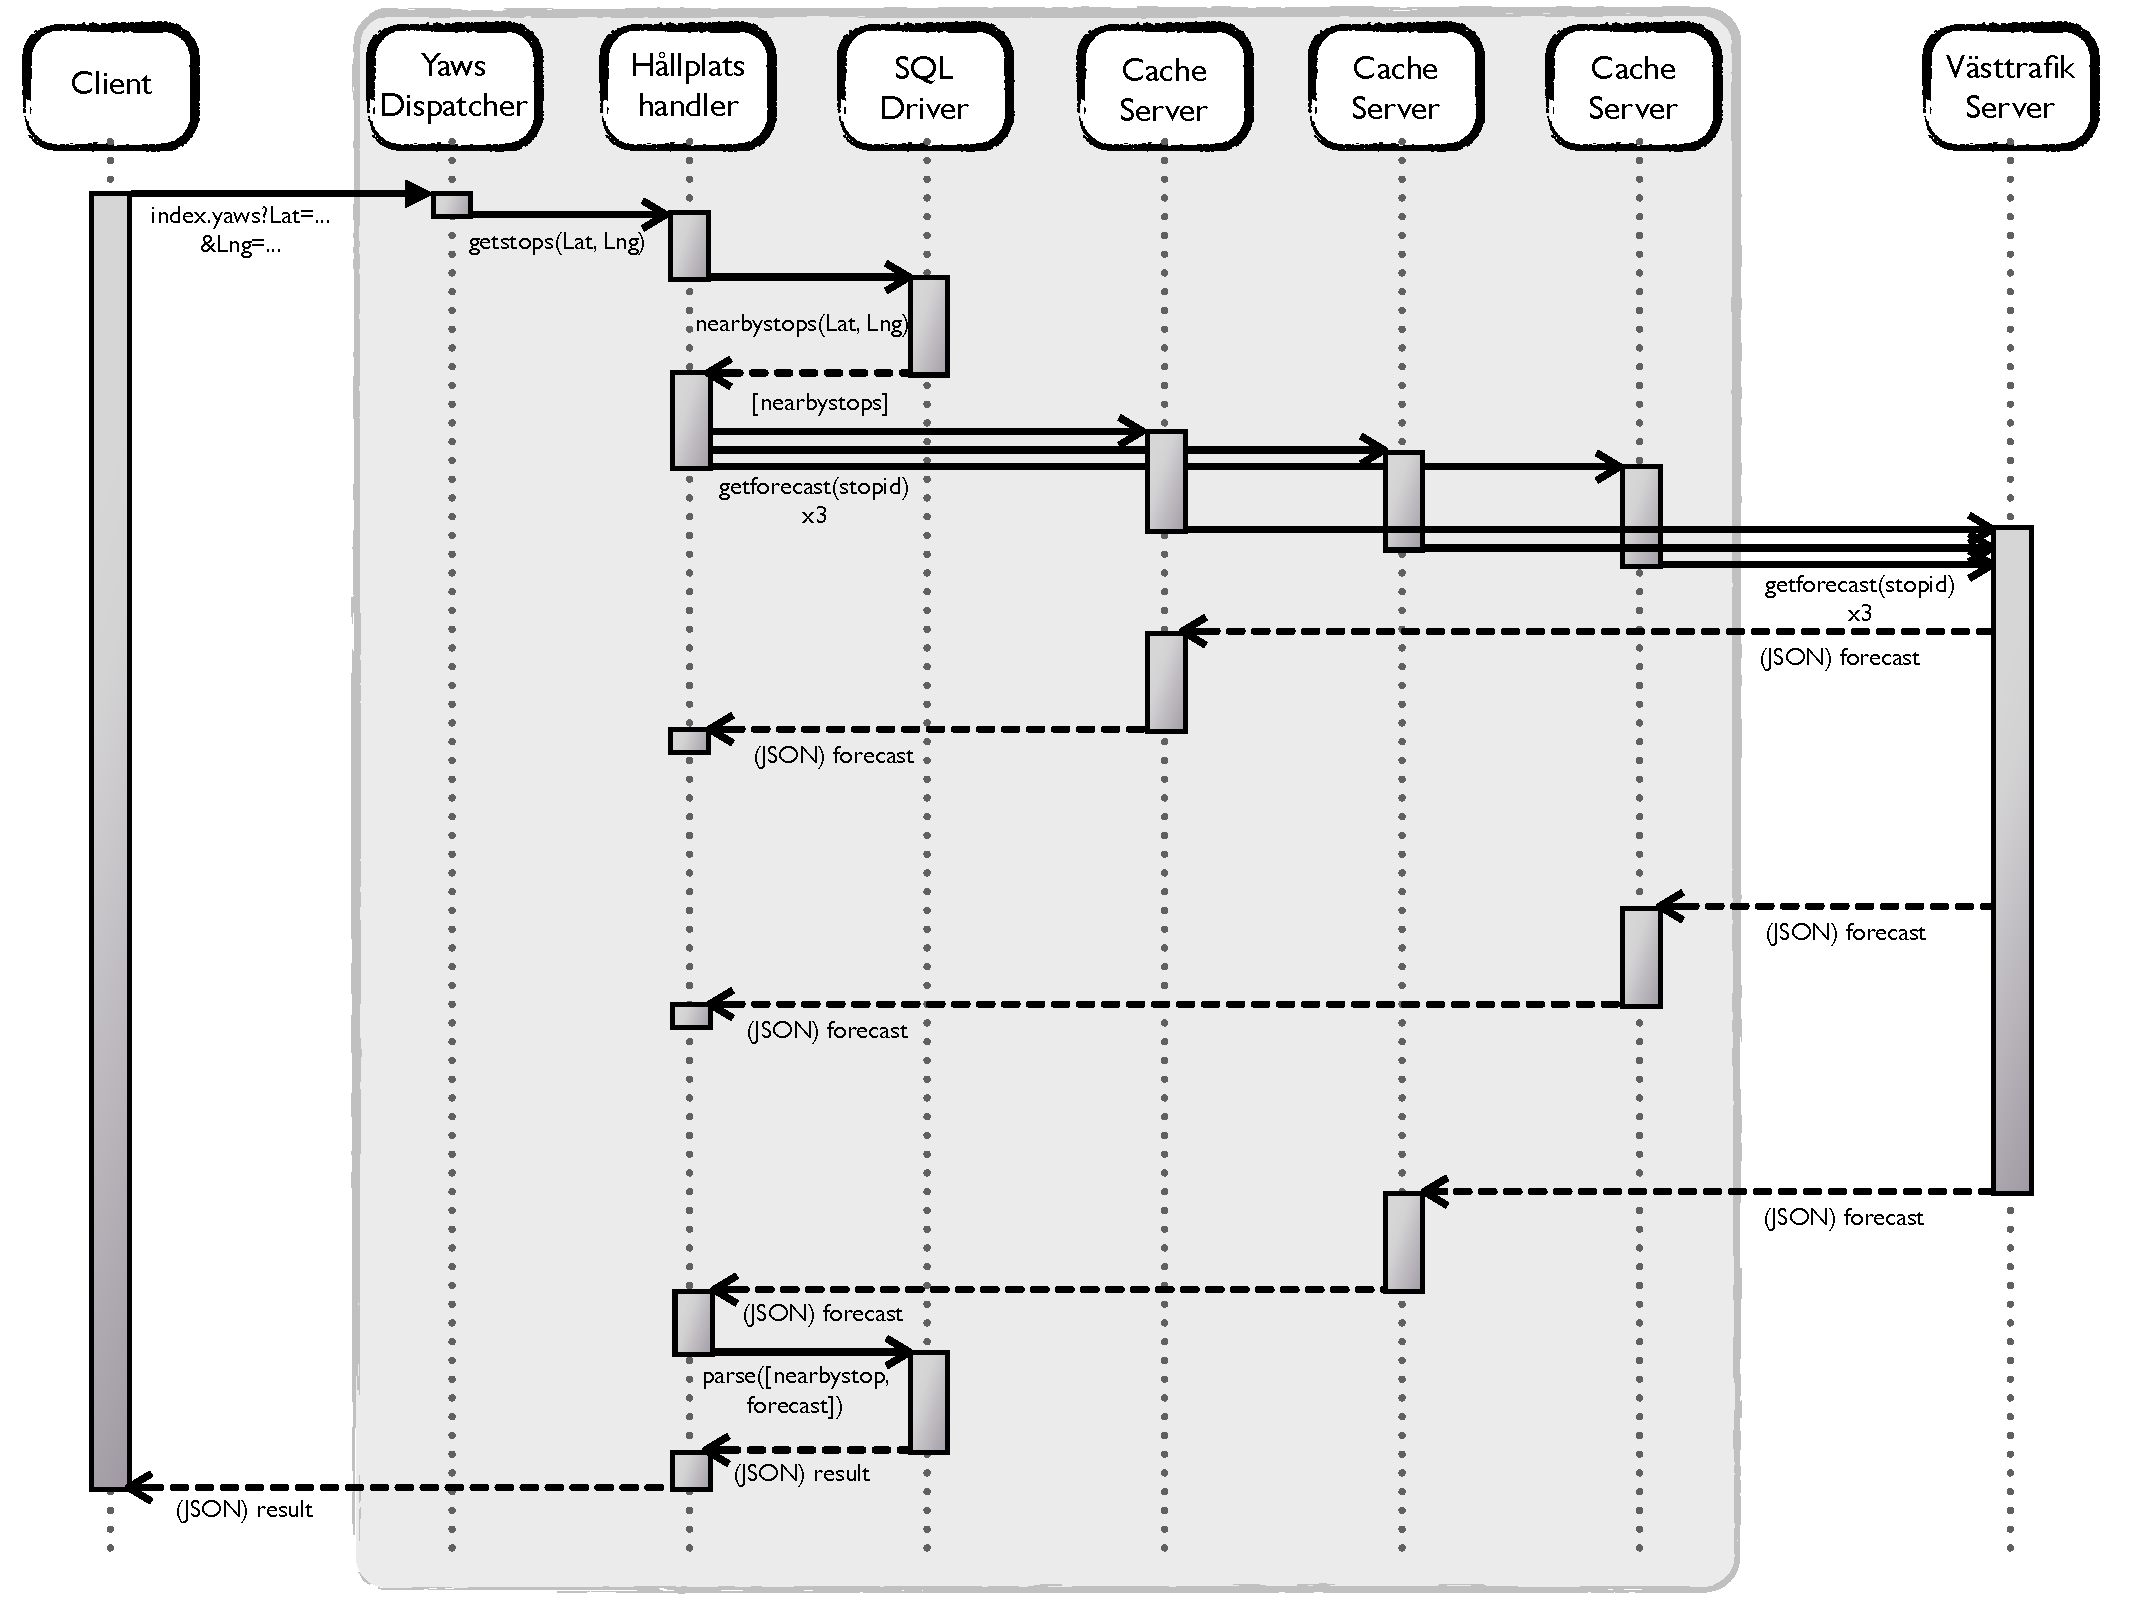
\includegraphics[scale=0.4]{pics/message_passing}
\caption{Simplified UML Sequential Diagram of a request}
\label{fig:message_passing}
\end{figure}


The application is hosted on a Debian machine (Ubuntu) with a Yaws webserver. Yaws is the Erlang alternative to Apache, and as such offers high availability and high scalability.

\begin{figure}[ht]
\center
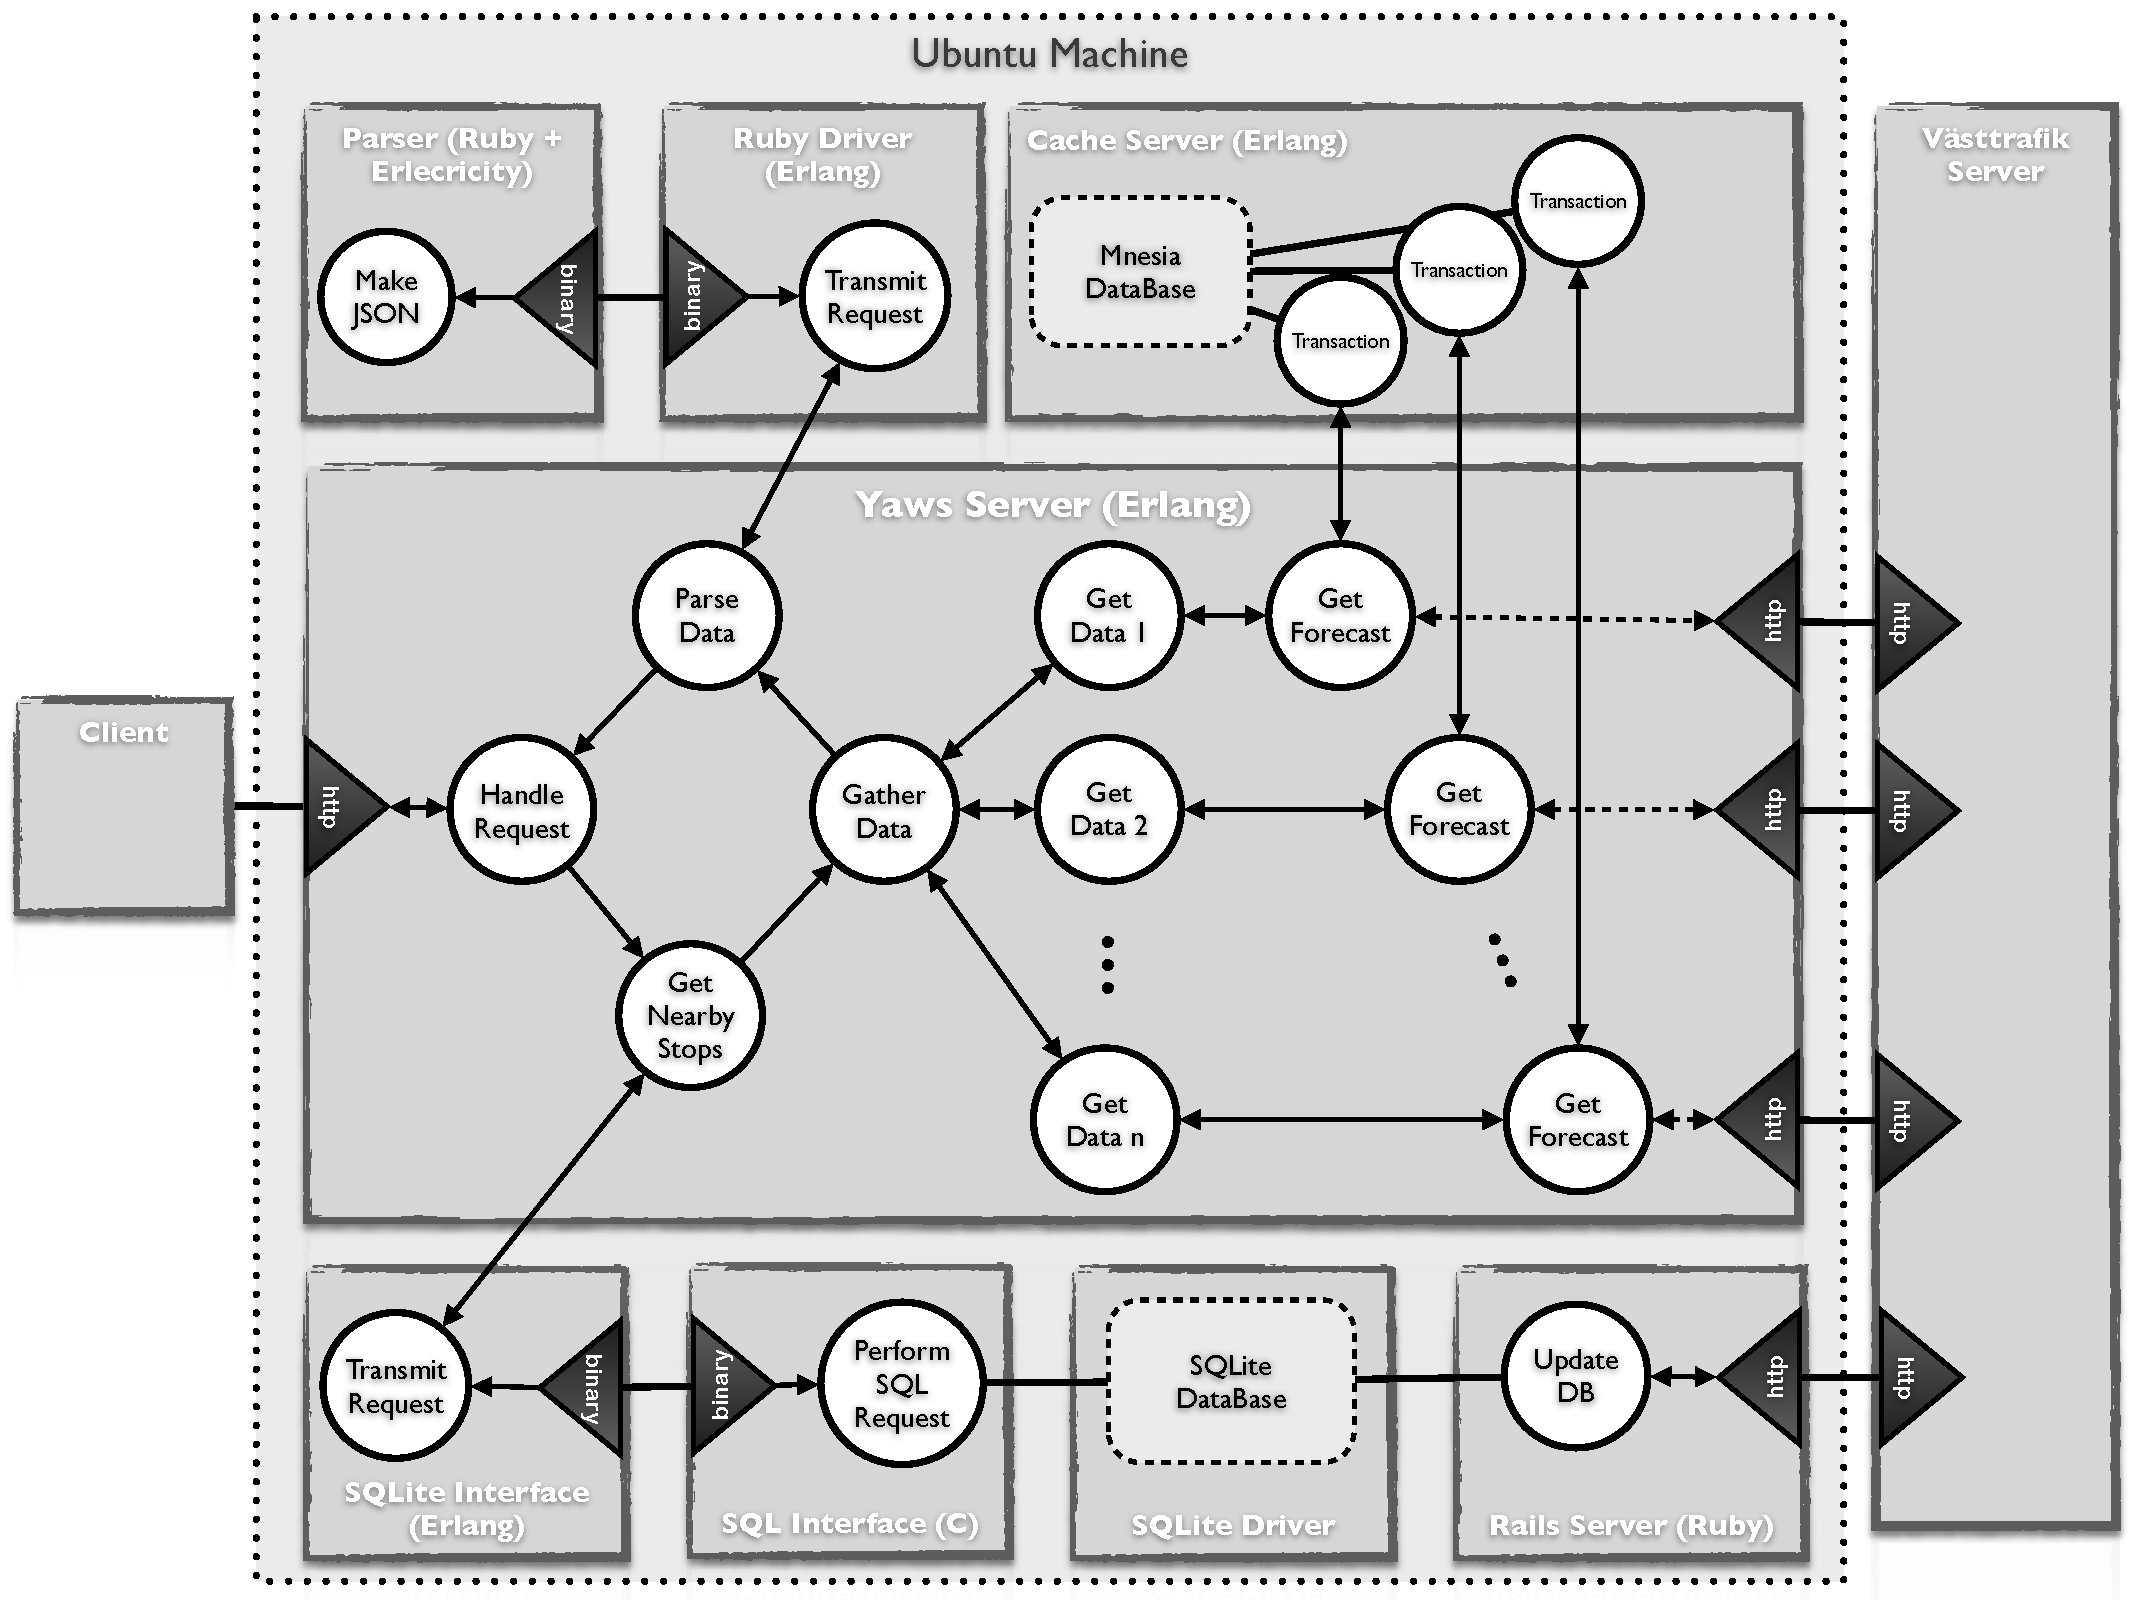
\includegraphics[scale=0.4]{pics/server_side}
\caption{Scheme of the Server Architecture}
\label{fig:server_architecture}
\end{figure}


Erlang is a functional programming language especially designed to handle high concurrency and distributed systems.  A large part of the application is therefore implemented in Erlang in order to take advantage of this.

But to make it easy to maintain and update, the more complex tasks are implemented in Ruby.

Ruby is a modern dynamic scripted language, and has been designed to make the developers happy. As such, it is a powerfull tool to implement complex algorithms painlessly.

%%%%%%%%%%%%%%%%%%%%%%%%%%%%%%%%%%%%%%%%%%%%%%%%%%%%%
\section{Implementation}

\subsection{Ruby}

Ruby is used to implement the SQL request to the database and to parse data. It is also used to maintain the database.

\subsection{Erlang}

Erlang is used to dispatch the lightweight processes, to perform the distant requests to Västtrafik and Storstockholms Locaktrafik, and also to take care of data caching by the mean of a Mnesia database.

%%%%%%%%%%%%%%%%%%%%%%%%%%%%%%%%%%%%%%%%%%%%%%%%%%%%%
\section{Results}

Everything works fine.

(give numbers)